\documentclass[runningheads,a4paper]{llncs}

\usepackage{amsmath}
\usepackage{graphicx}
\usepackage{subfig}
\usepackage{booktabs}
\usepackage{colortbl}
\usepackage{multirow}
\usepackage{epstopdf}
\usepackage{hyperref}
\usepackage{threeparttable}
\usepackage{booktabs}

\begin{document}

\title{A Machine Learning Approach for Instance Matching Based on Similarity Metrics}
\titlerunning{A Machine Learning Approach for Instance Matching}

\author{
    Shu Rong\inst{1}
    \and Xing Niu\inst{1}
    \and Evan Wei Xiang\inst{2}
    \and Haofen Wang\inst{1}
    \and Qiang Yang\inst{2}
    \and Yong Yu\inst{1}
}
\authorrunning{Shu Rong, Xing Niu, Evan Wei Xiang, Haofen Wang, etc.}

\institute{
    APEX Data \& Knowledge Management Lab, Shanghai Jiao Tong University\\
    \email{\{
        {\href{mailto:rongshu@apex.sjtu.edu.cn}{rongshu}},
        {\href{mailto:xingniu@apex.sjtu.edu.cn}{xingniu}},
        {\href{mailto:whfcarter@apex.sjtu.edu.cn}{whfcarter}},
        {\href{mailto:yyu@apex.sjtu.edu.cn}{yyu}}
    \}@apex.sjtu.edu.cn}
    \and Department of Computer Science and Engineering, Hong Kong University of Science and Technology, Hong Kong\\
    \email{\{
        {\href{mailto:wxiang@cse.ust.hk}{wxiang}},
        {\href{mailto:qyang@cse.ust.hk}{qyang}}
    \}@cse.ust.hk}
}
\maketitle


\begin{abstract}
The Linking Open Data (LOD) project is an ongoing effort to construct a global data space, i.e. the Web of Data. One important part of this project is to establish \texttt{owl:sameAs} links among structured data sources. Such links indicate equivalent instances that refer to the same real-world object. The problem of discovering \texttt{owl:sameAs} links between pairwise data sources is called \textit{instance matching}. Most of the existing approaches addressing this problem rely on the quality of prior schema matching, which is not always good enough in the LOD scenario. In this paper, we propose a schema-independent instance-pair similarity metric based on several general descriptive features. We transform the instance matching problem to the binary classification problem and solve it by machine learning algorithms. Furthermore, we employ some transfer learning methods to utilize the existing \texttt{owl:sameAs} links in LOD to reduce the demand for labeled data. We carry out experiments on some datasets of OAEI2010. The results show that our method performs well on real-world LOD data and outperforms the participants of OAEI2010.
\begin{keywords}
Linking Open Data, instance matching, similarity matric, machine learning, transfer learning
\end{keywords}
\end{abstract}

\section{Introduction}

Linked Data\cite{bizer2009linked} is a way to construct a global data space, the Web of Data, by interconnecting many structured data sources within the Linking Open Data\footnote{\url{http://linkeddata.org/}} (LOD) project. These data sources are published under the Resource Description Framework\footnote{\url{http://www.w3.org/RDF/}}(RDF). Each of them may contain millions of RDF triples.

The main idea of Linked Data is to construct typed links between different data sources. Such links describe the relationships between things so that users can browse data among sources by navigating along the links and agents can provide expressive query capabilities over the data on the web just like a local database. An important link is \texttt{owl:sameAs}\footnote{\url{http://www.w3.org/TR/2004/REC-owl-semantics-20040210/\#owl\_sameAs/}} which indicates that the two instances it links refer to the same real-world object. Different data sources may have different emphases in describing things. Various descriptions can be aggregated according to the \texttt{owl:sameAs} links.

Currently, there are more than 300 data sources in LOD while there were only twelve of them in 2007 when the project started. As more and more data sources emerge, there is an urgent demand to provide \texttt{owl:sameAs} links from the new data sources to the existing ones. At the same time, the existing links in LOD are not as extensive as one would hope\cite{hu2011self}. Instance matching is a practical idea for constructing such links. In general, the existing approaches for matching instances in LOD can be divided into two types. One is based on rules and the other is based on the similarity metric of instance pairs. Most of these methods do not always work well in the LOD scenario since they depend on the result of property matchings. Property matching links the properties from different data sources which have similar semantics such as \texttt{foaf:name} and \texttt{dc:title}. Property matching is not trivial since the data sources usually design their own ontologies to describe things. Furthermore, we noticed that although some properties in heterogeneous ontologies can not match, they have some connotative relationships. Their values may be worth considering for instance matching. For example, Freebase\footnote{\url{http://www.freebase.com/}} says that the \texttt{fb:profession} of Steve Jobs is \textquotedblleft Chief Executive Officer\textquotedblright  and his \texttt{fb:place\_of\_death} is \textquotedblleft Palo Alto\textquotedblright, whereas DBpedia\footnote{\url{http://www.dbpedia.org/}} says his \texttt{dbp:residence} is \textquotedblleft Palo Alto California\textquotedblright  and the information about \textquotedblleft Chief Executive Officer\textquotedblright  is in the text of the \texttt{dbp:abstract}. Such information will be ignored in property matching based methods, although it could be significant for human beings to judge whether the two Jobses match. We are inspired to explore the \textquotedblleft common-sense \textquotedblright  used for matching instances. The goal of this paper is to develop an automated instance matching method that is \textquotedblleft common\textquotedblright  and provides high accuracy. Such method should be independent of property matching to achieve \textquotedblleft commonality\textquotedblright .

In this paper, we employ machine learning models for instance matching based on some similarity metrics of instances. The matching instance pairs may have some common features in the similarity metrics of each pair. For example, two matching instances may share some significant words such as \textquotedblleft Palo Alto\textquotedblright  and \textquotedblleft Chief Executive Officer\textquotedblright  which we mentioned above, while the non-matching ones may not. Sharing some significant words is a common feature of the matching instance pairs here. We design a similarity vector independent of property matching to represent such features. Based on this vector, we train a learning model to classify the instance pairs as matching or non-matching. To minimize the demand for training data and promote the performance, we try to use existing instance matching information in LOD for help. A transfer learning method is applied to implement this idea.

We tried our approach on real LOD data sources which were chosen for IM@OAEI2010\footnote{\url{http://oaei.ontologymatching.org/2010/im/index.html}}. Our performance is better than the participating teams'. Another comparative experiment shows that the existing matching information can really help matching instances from the new data source pairs.

The following technical contributions are made:
\begin{itemize}
\item We utilize the values of non-matching properties for instance matching. Such values can be useful but are usually ignored by the existing instance matching approaches.
\item We propose a novel approach for instance matching which is independent of property matching with high accuracy.
\item We use existing \texttt{owl:sameAs} links to help match instances. Due to the heterogeneous ontologies constructed by various data sources, such information is hardly utilized in the existing instance matching approaches.
\end{itemize}

The remainder of this paper is structured as follows. Section \ref{sec:definition&framework} gives some definitions about instance matching and an overview of our proposed approach. Section \ref{sec:extraction} describes the feature extraction process. The selection of machine learning models is discussed in Section \ref{sec:learning}. Experimental results on the LOD datasets from LOD are reported in Section \ref{sec:experiments}. Some related work is discussed in Section \ref{sec:related}. Finally, Section \ref{sec:conclusion} concludes this paper and discusses future work. 
\section{Definition and Framework}
\label{sec:definition&framework}

\subsection{Problem Definition}
\label{sec:definition}

An instance consists of some property-value descriptions about a real-world object. A pair of distinct instances $a$ and $b$ match if they refer to the same object, denoted by $(a,b)\in\mathcal{R}$. In LOD, \texttt{owl:sameAs} links are established between matching instances. When establishing such links, we usually consider a pair of data sources each time.
\begin{definition}[Instance Matching]
Given two data sources $A$ and $B$ as input, the goal of instance matching is to compute the set $\mathcal{M}=\{(a,b)|(a,b)\in A \times B, (a,b)\in\mathcal{R}\}$.
\end{definition}
According to the definition of instance matching, the problem of finding matching instance pairs can be formalized as a binary classification problem.
\begin{definition}[Instance Matching as Binary Classification]
Given two data sources $A$ and $B$, the goal of instance matching is to find a classifier $\mathcal{C}:(a, b) \to\{-1, 1\}$ for $(a, b)\in A \times B$ such that $\mathcal{C}$ maps the non-matching instance pairs to class $-1$ and the matching ones to the class $1$.
\end{definition}
The binary classification problem can be solved by traditional machine learning algorithms, which require multidimensional features as the input. In the problem of instance matching, we extract a feature vector from each instance pair $(a, b)$.
\begin{definition}[Similarity Vector of Instance Pairs]
The n-dimensional feature vector $v$ of an instance pair $(a, b)$ consists of $n$ various similarities of instance $a$ and $b$. Dimension $v_i =d_i (a, b)$, where $d_i$ is the $i$th similarity metric function for $(a, b)$.
\end{definition}
The feature vector of an instance pair indicates the similarities of the two instances, which are computed by several metric functions. Some existing instance matching (record linkage\cite{elmagarmid2007duplicate}) approaches also extract such a feature vector for classification, while each $d_i$ computes the similarity of two values, one from each instance, that belong to a pair of matching properties (fields). Unlike these approaches, our similarity metric functions are based on the property-independent literal information extracted from each instance. The literal information $l=\{l_1 , l_2 , \dots , l_n\}$ is similar to a virtual document generated from an instance. For an instance pair $(a, b)$, a similarity metric function $d_i$ maps the extracted literal information pair $(l^a_i, l^b_i)$ to a real number in the range of $[0, 1]$.

\subsection{Framework}
\label{sec:framework}

\begin{figure}[t]
  \centering
  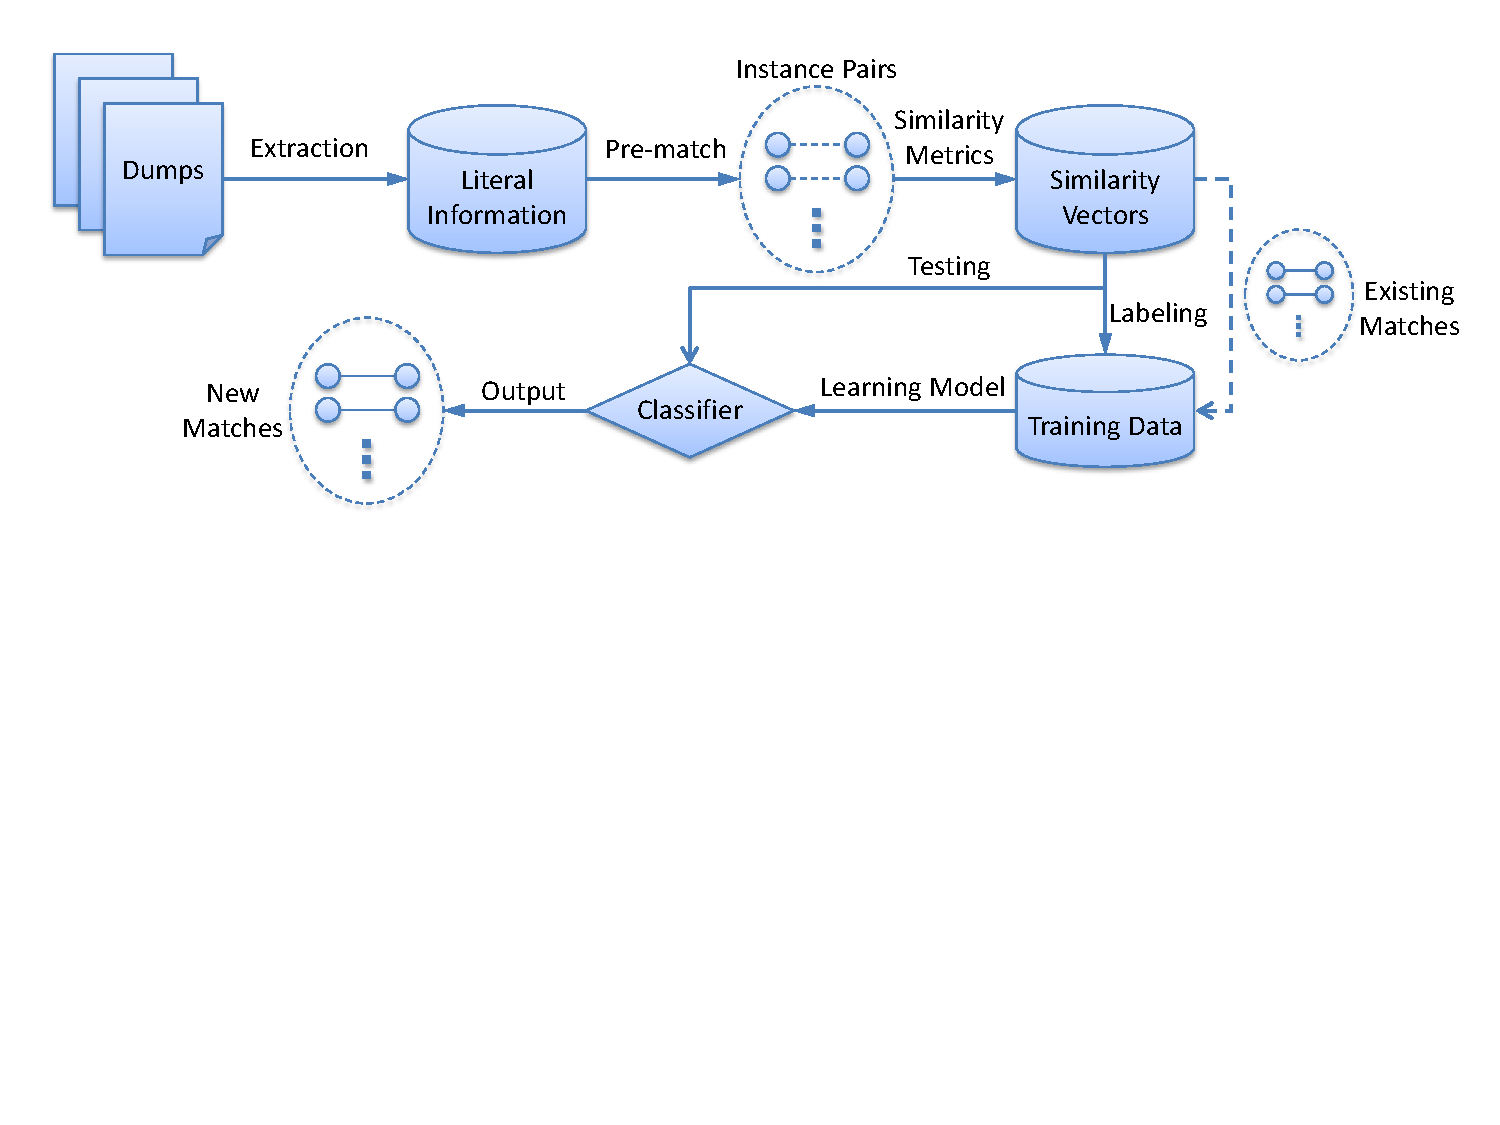
\includegraphics[width=1\textwidth]{figures/framework}
  \caption{Overview of the framework}
  \label{fig:framework}
\end{figure}
The framework of our approach is shown in Figure \ref{fig:framework}. We extract literal information for each instance from the property-value descriptions. To get sufficient literal information for the similarity metrics, we conduct the following preprocessing for each property-value pair:
\begin{itemize}
\item A real-world object may be represented by an instance or a piece of text. For consistency, if the value is a URI which represents another instance, we will replace it by the label of that instance. Most of the instances have a label value which usually belongs to the property \texttt{rdfs:label} or some other common properties\cite{ell2011labels}. If the label of an instance is unavailable, we can replace it by its text description.
\item We will also replace each property by its label. If the label is unavailable, we will use the last token (normalized) of the URI instead, e.g., \textquotedblleft place of death \textquotedblright for \texttt{fb:place\_of\_death}.
\end{itemize}
For data sources $A$ and $B$ which contain $|A|$ and $|B|$ instances respectively, there are $|A|\times|B|$ possible instance pairs. This is unacceptable since both $|A|$ and $|B|$ can be one million or even larger. We use a simple pre-match method to sift the possible matching pairs. An inverted index is built for instances of some key words in their descriptions. The instances sharing the same keys in the index are considered to be candidate matching instances. Our preliminary experiments show that this sifting method can greatly reduce the number of pairs  to test for a match, without losing much recall (the recall is over $0.9$).

After preprocessing and literal information extraction, we compute the similarity vectors for the candidates. To train a binary classifier based on the similarity vectors, we need to label some of them into class -1 (non-matching) or class 1 (matching). Thus the problem of instance matching can be solved by classifying the unlabeled instance pairs. The existing matching instance pairs in LOD can be considered as labeled data which may help to train the classifier. We employ a transfer learning algorithm to improve the effect of the helping.

\section{Feature Extraction}
\label{sec:extraction}

We extract some property-independent information from each instance and then compute the similarity vectors for instance pairs based on this information. Since the performance of a machine learning algorithm depends a lot on the quality of feature extraction, the work in this section is vital for the next step.

\subsection{Literal Information Extraction}
\label{sec:literal}

We extract several sets of literal information from each instance. The first is the text information set $l_{label}$, that is the label of an instance. The label is the human-readable name for an instance, such that it can help people to identify the real-world object. So labels are discriminative for instance matching. Next, we extract the remaining text information from the instance. These sets are divided into two parts. One is $l_{property}$ which consists of the text information from properties. The other is the text information from the values. The number of words in a value has a certain meaning. If the value only contains one word, this word can be a specific symbol such as the ISBN for a book. If the number of words is small, these words are likely to be the name of something, e.g. "Palo Alto". If there are a lot of words in the value, they may be a text description. These three kinds of values may play different roles in the problem of instance matching. So we extract them as $l_{single}$, $l_{short}$ and $l_{long}$ respectively.

Besides the large amount of text information, there are also other types of literal information in the instance descriptions. The common ones we used are dates, numbers and links. In contrast to the text information, these types of literal information are more useful for instance matching. If two instances share some dates, numbers or links, they are likely to match. So we additionally extract them as $l_{date}$, $l_{number}$ and $l_{link}$. Note that:
\begin{itemize}
\item There are many forms of dates. For convenience, we only extract the year part of each date and the other parts are treated as text.
\item Some dates and numbers may be included in the texts. We use meticulous string processing to find them.
\end{itemize}

\subsection{Similarity Metrics}
\label{sec:metric}
Different similarity metric functions are used for different types of literal information. As shown in Table \ref{tab:metric}, a 12-dimensional similarity vector is generated for each instance pair.
\begin{table}[t]
\caption{Overall Statistics on Extraction Results}
\label{tab:metric}
\centering
\begin{tabular}{c|c|c}
  \toprule
  Dimension Num & Metric Function & Combination of Literal Information\\
  \midrule
    1 & $\mathrm{IdfSim}$ & $l_{single}$ \\
    2 & $\mathrm{TopIdfSim}$ & $l_{single}$ \\
    3 & $\mathrm{IdfSim}$ & $l_{single}\cup l_{short} \cup l_{label}$ \\
    4 & $\mathrm{TopIdfSim}$ & $l_{single}\cup l_{short} \cup l_{label}$ \\
    5 & $\mathrm{CosSim}$ & $l_{single}\cup l_{short} \cup l_{label} \cup l_{property} \cup l_{long}$ \\
    6 & $\mathrm{IdfSim}$ & $l_{single}\cup l_{short} \cup l_{label} \cup l_{property} \cup l_{long}$ \\
    7 & $\mathrm{TopIdfSim}$ & $l_{single}\cup l_{short} \cup l_{label} \cup l_{property} \cup l_{long}$ \\
    8 & $\mathrm{EditSim}$ & $l_{label}$ \\
    9 & $\mathrm{CountSim}$ & $l_{label}$ \\
    10 & $\mathrm{CountSim}$ & $l_{date}$ \\
    11 & $\mathrm{CountSim}$ & $l_{number}$ \\
    12 & $\mathrm{CountSim}$ & $l_{link}$ \\
  \bottomrule
\end{tabular}
\end{table}

For the text information, we use three functions, $\mathrm{CosSim}$, $\mathrm{IdfSim}$ and $\mathrm{TopIdfSim}$. $\mathrm{CosSim}$ is a common similarity metric for texts. It computes the $\mathrm{TF}\cdot\mathrm{IDF}$\cite{cohen1998integration} weights for the words from two word sets and then computes their \textit{cosine similarity}. Furthermore, in the particular problem of instance matching, the $\mathrm{IDF}$ weights are more important. Some common words or common words for the domain may appear frequently in the descriptions of many instances. These words with high $\mathrm{TF}$ weights but low $\mathrm{IDF}$ weights do not much help match instances. While if a word only appears once in each data source, the two instances that contain it are likely to match. According to this idea, $\mathrm{IdfSim}$ and $\mathrm{TopIdfSim}$ are designed based on the $\mathrm{IDF}$ weights of words. $\mathrm{IdfSim}$ is similar to $\mathrm{CosSim}$ which just removes the $\mathrm{TF}$ weights. For word sets $T_1$ and $T_2$, $\mathrm{TopIdfSim}$ computes the similarity of $W_1$ and $W_2$, where $W_i$ is a subset of $T_i$ which consists of the words with highest $\mathrm{IDF}$ weights in $T_i$. It is computed by:
\begin{equation}
\mathrm{TopIdfSim}(T_1, T_2) = \frac{\sum_{w\in W_1\cap T_2}{}{\mathrm{IDF}(w)} + \sum_{w\in W_2\cap T_1}{}{\mathrm{IDF}(w)}}
                        {\sum_{w\in W_1}{}{\mathrm{IDF}(w)} + \sum_{w\in W_2}{}{\mathrm{IDF}(w)}}
\end{equation}
These three similarity metric functions act on the combinations of the extracted word sets of text information. The combining strategy is based on the relaxed inclusion relation of these word sets from different instances, that is $l_{single}$ may be included in $l_{short}$ or $l_{label}$, and $l_{long}$ main contains all the other word sets.

Among the sets of text information, $l_{label}$ is different from the others in two ways as follows:
\begin{enumerate}
    \item We only extract one label for each instance; so it can be treated as a set of words or a string.
    \item Since each word in a label can be significant for recognizing the entity, to match two instances, the matching words of their labels are more important than the non-matching ones.
\end{enumerate}
So we design another two similarity metrics for $l_{label}$, which are $\mathrm{EditSim}$ and $\mathrm{CountSim}$.
\begin{equation}
\mathrm{EditSim}(l_{label}^a, l_{label}^b) = 1 - \frac{\mathrm{EditDistance}(S_a, S_b)}{\mathrm{Max}(|S_a|, |S_b|)}
\end{equation}
Where $S_a$ stands for the string form of $l_{label}^a$ and $\mathrm{EditDistance}(S_a, S_b)$ is a classical string-distance measure, which represents the minimum number of editing operations needed to make $S_a$ and $S_b$ the same. Each operation can be deleting a character, inserting a character or changing a character in either $S_a$ or $S_b$.
\begin{equation}
\mathrm{CountSim}(l_{label}^a, l_{label}^b) = \frac{1 - 2^{-|\{w|w\in l_{label}^a\cap l_{label}^b\}|}}
                        {1 - 2^{-\lceil (|l_{label}^a|+|l_{label}^b|)/2 \rceil}}
\end{equation}

The literal information sets of dates, numbers and links also have the second characteristic of the labels. So we use $\mathrm{CountSim}$ on them to generate similarities. Note that two numbers are considered to be the same one if their difference is lower than a threshold.


\section{Learning Algorithms}
\label{sec:learning}

After extracting the feature vectors, we can train the classifier for instance matching. There are many machine learning algorithms for the binary classification problem. We need to carefully choose the appropriate ones according to the characteristic of the input data.

\subsection{Basic Learning Model}

In our problem, the input data may contain millions instance pairs. So some methods with high time cost such as \textit{Neural Networks} and \textit{SVM} with a complex kernel are eliminated. After observing the feature space via a preliminary experiment, we found that the data of the two classes are not linearly separable. A typical example is shown in Figure \ref{fig:space}. $x$ and $y$ are two dimensions of the similarity vector. The positive and negative regions represent the two classes. Figure \ref{fig:space} indicates that for a similarity vector, if $x$ is greater than a threshold, it belongs to the class of matching instance pairs when $y$ is large, but if $x$ is less than the threshold, it belongs to the matching class when $y$ is small. From the perspective of each single dimension, this situation does not meet our intuition. The value of each dimension describes the similarity of two instances based on a certain metric. The higher the value is, the more likely they will match. But from the perspective of the correlation between the dimensions, such a situation is reasonable. We will give an example to explain it.

\begin{figure}[t]
  \centering
  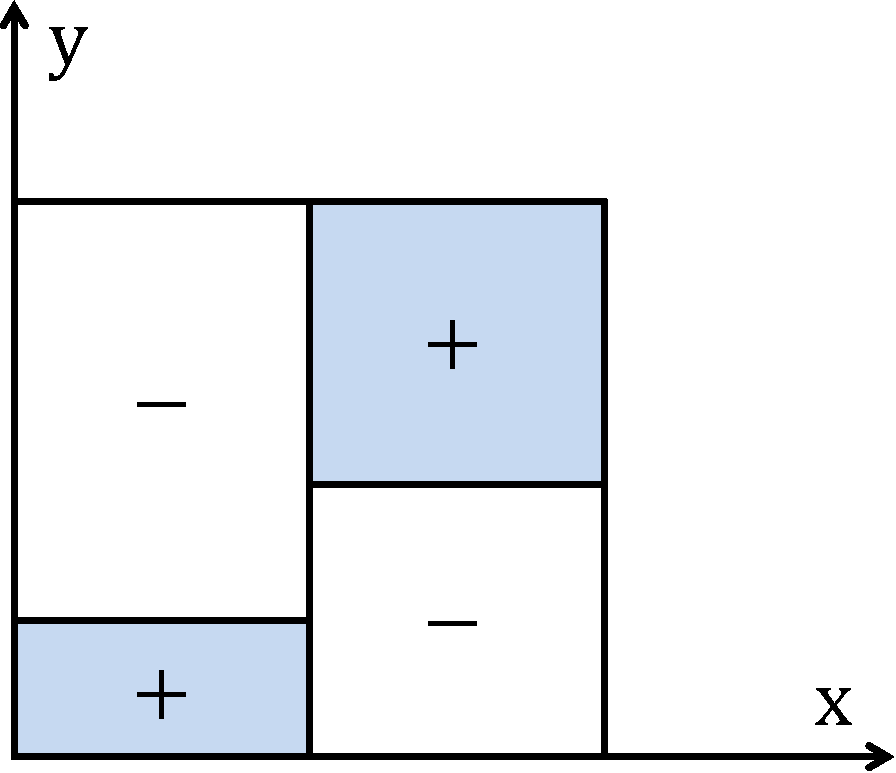
\includegraphics[width=0.3\textwidth]{figures/space}
  \caption{A typical example of the feature space}
  \label{fig:space}
\end{figure}

On one hand, given two instance pairs $(p_1, p_2)$ and $(q_1, q_2)$, their similarity vectors are $u$ and $v$. We assume that $u_6=v_6=0.3$, $u_5=0.1$ and $v_5=0.3$ where $u_i$($v_i$) stands for the $i$th dimension of the similarity vector $u$($v$). Probably, instance $p_1$ consists of long texts and instance $p_2$ consists of short texts or single words, so that $u_5=0.1$. While $q_1$ and $q_2$ both consist of long texts which share some common (for the domain) words, so $v_5=0.3$. Furthermore, $p_1$ and  $p_2$ may share some important words such that $u_6=0.3$. While the value $0.3$ of $v_6$ may be obtained by the common words. According to the inference above, $(p_1, p_2)$ is likely to match while $(q_1, q_2)$ is not. On the other hand, an instance pair with large values of both dimensions $5$ and $6$ is likely to match.

Since the feature space is so complex, some linear classifiers are inapplicable here, e.g. \textit{linear regression} and \textit{SVM}. Actually, the dimensions of our similarity vector have some implicit associations, especially the ones generated from the same combination of text sets. So the model we needed should properly handle such associations for classification.

Consider the \textit{decision tree} model: A decision tree is a binary tree. Each non-leaf node $t$ in the tree has a dimension-number $k_t$ and a threshold $\sigma_t$ and each leaf node has a label of one of the two classes. When a testing vector is sent to a non-leaf node $t$, it will be sequentially sent to a child node according to whether the value of $k_t$th dimension of the vector is greater than $\sigma_t$. So a testing vector will be sent to the root of the tree and finally get to a leaf node. The label of the leaf node will be the class the vector belongs to. The vectors which arrive at node $t$ have passed the ancestors of $t$, i.e. $A_t$. In this way, the associations between dimension of $k_t$ and the dimensions of $\{ k_a | a\in A_t\}$ are taken into consideration for classification.

\subsection{AdaBoost with Random Forest}

\textit{AdaBoost}\cite{freund1995desicion} is the predecessor of the transfer learning algorithm we will use. It combines several weak classifiers to get a powerful classifier via an iterative process. In each round of iteration, it employs a basic learning model to train a weak classifier with the current weighted examples. Then it increases the weights of the examples which are incorrectly classified by the weak classifier, so that these \textquotedblleft difficult\textquotedblright ones will be classified better in the following rounds. In this way, \textit{AdaBoost} may improve the performance of the basic learning model.

We found that some classical decision tree algorithms do not show good performance working with \textit{AdaBoost}. In the training phase, the decision tree will continually grow to satisfy the training data. Since \textit{AdaBoost} combines the examples from source and target domain for training, the trained tree-classifier will achieve good performance on both source and target domain examples. This leads to a situation where few incorrectly classified examples can be found during the iterations and the weights are hardly changed.

To solve this problem, we choose a specific decision tree model, \textit{Random Forest}. A random forest contains several decision trees. Each of them is trained with a newly constructed training set, which is chosen by randomly picking some examples with replacement from the whole training data. The classification result of the random forest is a voting result of these trees. Due to the chosen strategy of the training set, most trees will only be good at classifying the examples in the dominating distribution. The remaining examples will be incorrectly classified so that they will be reweighted. Our preliminary experiments show that as a basic learning model of \textit{AdaBoost}, \textit{Random Tree} is superior to the other decision tree models, e.g. \textit{J48Tree}\cite{loh2008classification}.

\subsection{Transfer Learning}

To train an efficient classifier, a number of training examples are needed and should be labeled manually. To reduce the manual work, we want to utilize the existing matching instance pairs in LOD for help. But most machine learning methods work well only under the assumption that the training and testing data are drawn from the same feature space and the same distribution\cite{pan2010survey}. Training data which is generated from the existing matching instance pairs does not meet this requirement. \textit{Transfer learning}\cite{pan2010survey} can utilize the data from different distributed domains (\textit{source domain}) to help the target task, thus reducing the need for training data in the \textit{target domain} (the domain of testing data).

There are two main kinds of transfer learning methods: the \textit{instance-transfer} and the \textit{feature-representation-transfer}. The former assumes that the feature spaces of the source and target domain are the same while the distributions of the data from the two domains are different. Such methods try to find examples from the source domain which can be reused to help the target domain task. The latter assumes that the feature spaces of the source and target domain are different. Such methods focus on finding the \textquotedblleft good\textquotedblright  common features which reduce the difference between the source and target domains and the error of classification.

The property matching independent similarity vectors we generated naturally compose a common feature space for all the data source pairs. So we employ \textit{TrAdaBoost}\cite{dai2007boosting} for help, which is a classical algorithm for \textit{instance-transfer} learning. \textit{TrAdaBoost} is an extension of the \textit{AdaBoost}\cite{freund1995desicion} algorithm. It assumes that the feature spaces of source and target domain are the same while the distributions of the data from the two domains are different. Due to the different distributions, some of the source domain data may be helpful in training the classifier for the target domain but some of it may not be and could even be harmful. \textit{TrAdaBoost} iteratively adjusts the weighting of the source domain data to reduce the effect of the \textquotedblleft bad\textquotedblright  source data. In each round of iteration, \textit{TrAdaBoost} trains the basic classifier on the weighted source and target data. The source domain examples which are classified incorrectly by the classifier are considered to be the ��bad�� source data, so their weights are reduced. Meanwhile, \textit{TrAdaBoost} uses the same strategy as \textit{AdaBoost} that is to increase the weights of the incorrectly classified examples in the target domain.

\textit{Random Forest} is a suitable basic learning model for \textit{TrAdaBoost}, as well as for \textit{AdaBoost}. The interface of \textit{TrAdaBoost} is generic. We can directly apply it on the problem of instance matching by treating the instance pairs from a pair of data sources, which are to be matched, as the target domain, and the existing matching information between another pair of data sources as the source domain. But not all the source domains can help to train the classifier on the target domain via \textit{TrAdaBoost}. A source domains can be harmful if its distribution is quite different from that of the target domain.

The problem of how to automatically choose a helpful source domain has not been theoretically solved yet\cite{eaton2011selective}. Intuitively, the more similar the distributions of the two domains are, the more likely the source domain can help. In the problem of instance matching, the distribution of a domain is decided by the heterogeneity between the ways of describing objects which are used by the data sources (We call it describing heterogeneity for short). So when we want to match the instances of a data source pair $(A, B)$, we should use another pair $(C, D)$ for help, such that the describing heterogeneities of $(A, B)$ and $(C, D)$ are similar.

\section{Experiments}
\label{sec:experiments}

First, we will show the experimental results of our proposed approach without transfer learning. We use the dataset provided by the data interlinking track of IM@OAEI2010 and compare our approach with the participants'. We chose this dataset because many others are not from LOD. Then we will give some comparative experiments to show whether a source domain we chose from LOD is helpful to instance matching via transfer learning.

\subsection{Without Transfer Learning}

The goal of the data interlinking track of IM@OAEI2010 is to find all the \texttt{owl:sameAs} links from four data sources to the ones in LOD. These four data sources are also in LOD; they are:
\begin{itemize}
\item Sider\footnote{\url{http://sideeffects.embl.de/}}, about some drugs and their effects.
\item DrugBank\footnote{\url{http://www.drugbank.ca/}}, about drugs and their chemical, pharmaceutical and pharmacological information.
\item DiseaSome\footnote{\url{http://http://diseasome.kobic.re.kr/}}, about disorders and genes.
\item DailyMed\footnote{\url{http://dailymed.nlm.nih.gov/}}, about marketed drugs and chemical structure, mechanism of action, indication, usage, contraindications and adverse reactions for the drugs.
\end{itemize}
These data sources are already linked to LOD and the existing links will be treated as the standard answers. The well-known \textit{Recall}, \textit{Precision} and \textit{F-Measure} are used for evaluation.

Two teams, ObjectCoref and RiMOM took part in this track. Their reports of results can be found in \cite{wang2010rimom} and \cite{hu2010objectcoref}. ObjectCoref\cite{hu2011self} uses a self-learning framework to iteratively extend a kernel of matching instances. In each round of iteration, the most discriminative property-value pair is learned from the kernel for the further matching. RiMOM\cite{li2009rimom} is a multi-strategy ontology matching framework. It combines three strategies when facing an instance matching problem.
\begin{enumerate}
\item Edit distance between labels of two instances.
\item Cosine of the $\mathrm{TF}\cdot\mathrm{IDF}$ vectors for the text description of the instances to match.
\item Cosine of the $\mathrm{TF}\cdot\mathrm{IDF}$ vectors for the text description of the instances related to the ones to match.
\end{enumerate}

\begin{table}[t]
\caption{Compare with the Participants of IM@OAEI2010}
\label{tab:oaei}
\centering
\begin{tabular}{c|c|c|c|c}
  \toprule
  Data Set & Approach & Recall & Precision & F-Measure  \\
  \midrule
    Sider-DrugBank & ObjectCoref & 0.996 & 0.302 & 0.464 \\
    & RiMOM & 0.342 & 0.961 & 0.504 \\
%    & Random Forest & 0.852 & 0.882 & 0.866\\
    & AdaBoost & 0.859 & 0.952 & \textbf{0.903} \\
  \midrule
    Sider-DiseaSome & ObjectCoref & 0.668 & 0.837 & 0.743 \\
    & RiMOM & 0.315 & 0.837 & 0.458 \\
%    & Random Forest & 0.820 & 0.851 & \textbf{0.835}\\
    & AdaBoost & 0.726 & 0.875 & \textbf{0.794} \\
  \midrule
    Sider-DailyMed & ObjectCoref & 0.999 & 0.548 & 0.708 \\
    & RiMOM & 0.567 & 0.706 & 0.629 \\
%    & Random Forest & 0.842 & 0.669 & \textbf{0.746} \\
    & AdaBoost & 0.672 & 0.805 & \textbf{0.733} \\
  \midrule
    Sider-DBpedia & RiMOM & 0.482 & 0.717 & 0.576 \\
%    & Random Forest & 0.690 & 0.258 & 0.375 \\
    & AdaBoost & 0.643 & 0.639 & \textbf{0.641} \\
  \midrule
    DailyMed-DBpedia & RiMOM & 0.246 & 0.293 & 0.267 \\
%    & Random Forest & 0.321 & 0.414 & 0.362 \\
    & AdaBoost & 0.373 & 0.377 & \textbf{0.375} \\
  \bottomrule
\end{tabular}
\end{table}

In Table \ref{tab:oaei}, we give the results of matching instances for each data source pair. RiMOM also gave their results on some other data source pairs which are not shown here, since we can not find the dumps of those data sources. For each testing data source pair, we randomly labeled $5\%$ of the similarity vectors as training data (no more than 2000 for these datasets). Obviously, our proposed approach works better than ObjectCoref and RiMOM on these datasets.

For ObjectCoref, the process of learning discriminative property-value pairs depends on the lax matches of properties from different data sources. From the report of ObjectCoref\cite{hu2010objectcoref}, we can see that the matching properties found for these datasets are mainly about names and aliases. By analyzing the data, we find that Sider, DrugBank and DayliMed contain a lot of aliases for each instance, while DiseaSome does not. Furthermore, some non-matching instances have similar aliases. So ObjectCoref got high recall and low precision on Sider-DrugBank and Sider-DailyMed, but low recall and high precision on Sider-DiseaSome. In general, ObjectCoref did not get good performance since the properties of names and aliases do not match well. In contrast, RiMOM is a property matching independent approach. But the similarity metric that combines the three strategies is not accurate enough for instance matching.

%In most cases, \textit{AdaBoost} can improve the performance of the basic learning model, which has met our expectations.
We noticed that our proposed approach has an enormous advantage on the data set Sider-DrugBank. The probable reason is that we can make use of the names and aliases for instance matching. Our approach eliminates the ill effects of the duplicate names by giving them low $\mathrm{IDF}$ weights.

\subsection{With Transfer Learning}

\begin{table}[t]
\caption{Transfer GeoNames-DBpedia to LinkedGeoData-DBpedia}
\label{tab:transfer}
\centering
\begin{tabular}{c|c|c|c}
  \toprule
    Training Examples & AdaBoost & AdaBoost(Source) & TrAdaboost \\
  \midrule
    900\tnote{1} & 0.284 & 0.372 & \textbf{0.378} \\
    1500 & 0.383 & 0.396 & \textbf{0.432} \\
    3000 & 0.444 & 0.416& \textbf{0.458} \\
    6000 & \textbf{0.524} & 0.450 & 0.516 \\
    15000 & \textbf{0.544} & 0.491 & 0.536 \\
  \bottomrule
\end{tabular}
\end{table}

We choose GeoNames\footnote{\url{http://www.geonames.org/}}, LinkedGeoData\footnote{\url{http://linkedgeodata.org/}} and DBpedia as the datasets for the experiments on transfer learning. GeoNames and LinkedGeoData are data sources in LOD. Both of them are about geographic information and have \texttt{owl:sameAs} links to DBpedia. GeoNames and LinkedGeoData have similar behaviors in describing real-world objects. So the the describing heterogeneities of GeoNames-DBpedia and LinkedGeoData-DBpedia are similar. We try to use the information on the existing matching instances between GeoNames and DBpedia to help matching LinkedGeoData and DBpedia.

The result is shown in Table \ref{tab:transfer}. \textbf{AdaBoost} denotes the \textit{AdaBoost} model applied only on the training data from the target domain (LinkedGeoData-DBpedia). \textbf{AdaBoost(Source)} and \textbf{TrAdaBoost} respectively denote the \textit{AdaBoost} and \textit{TrAdaBoost} model applied on the training data from both domains. \textbf{Training Examples} denotes the number of training instance pairs we labeled in the target domain. 900 examples are about $0.01\%$ of all the pre-matching instance pairs between LinkedGeoData and DBpedia. We can see that the source domain we chose is really helpful via \textit{TrAdaBoost}. But directly using the source domain for training can be harmful. Furthermore, the less training data there is in the target domain, the more the source domain can help. If there is efficient training data in the target domain, the source domain is entirely useless. These experimental results match our intuition about transfer learning.

\section{Related Work}
\label{sec:related}

Although the problem of instance matching has emerged along with the development of LOD in recent years, a similar problem, \textit{Record linkage}, was examined much earlier. Thus a lot of relevant approaches have been proposed.

\subsection{Record Linkage}

\textit{Record linkage}, also known as \textit{duplicate detection} or \textit{object identification}, is a classical problem in the area of databases. The goal of record linkage is to determine the pairs of records that are associated with the same entity across various data sets. It is similar to the instance matching problem. For more than five decades, the traditional database community has discussed this problem a lot. Some surveys can be found in \cite{winkler1999state}, \cite{winkler2006overview} and \cite{elmagarmid2007duplicate}.

The early approaches focus on similarity metrics for single field (column) matching. Many of them are even widely used today, such as edit distance, \textit{Q}-gram distance, etc. The similarity vector in our work is based on $\mathrm{TF}\cdot\mathrm{IDF}$\cite{cohen1998integration} and its variants.

The approaches for multi-field matching are mainly based on probabilistic models, developed by the machine learning community. The learning methods were applied on record linkage by extracting the feature vector of similarities from the comparable fields. Such approaches classify the record pairs as matching or not, employing CART\cite{cochinwala2001efficient}, SVM\cite{bilenko2003adaptive} and so on. Semi-supervised, active and unsupervised learning algorithms have been proposed to reduce the demand for training data. Unlike the properties of linked data sources, the number of fields in a record linkage problem is usually quite small. Thus the comparable fields can be easily found manually. So the data base community doesn't pay attention to the problem known as \textit{Structural heterogeneity}. A simple schema-independent method has also been proposed which treats the whole record as one large field. But experiments in \cite{bilenko2003adaptive} show that SVM based on the similarity metric of multiple comparable fields usually outperforms it. It's easy to see that such an elaborate similarity metric benefits record linkage when the fields can well match. Some distance-based methods which have also been proposed for for multi-field matching do not employ machine learning algorithms\cite{guha2004merging}\cite{ananthakrishna2002eliminating}, but the distance measures are also based on schema matching.

Some other work focuses on postprocessing. The main idea is that the matching relations between records or fields should be consistent\cite{bansal2004correlation}\cite{pasula2002identity}. Such methods based on graph model can play an important role in instance matching problems as the linked data settings are more structured. They are complementary to our proposed work which uses only the literal information.

\subsection{Instance Matching}

Some of the existing links in LOD are discovered manually with some tools. One well-known instance matching tool is the Silk Link Discovery Framework\cite{volz2009discovering} which allows setting link specifications for given data sources. Domain related knowledge is required to design such specifications.

The automatic instance matching approaches are often domain specific or property matching dependent. The approach proposed in \cite{sleeman2010machine} matches the FOAF instances using SVM. Since all of the instances are described with FOAF, the features for classification are easily determined according to the limited number of properties. More domain-specific approaches can be found in \cite{raimond2008automatic} and \cite{sleeman2010computing}. Among the domain-independent approaches, \cite{hogan2007performing} matches instances according to their inverse functional properties (IFP). Such properties are not sufficient in LOD, so \cite{hogan2010some} tries to find more IFPs with a statistical method. ObjectCoref\cite{hu2011self} employs a self-learning framework to iteratively find the discriminative property-value pairs for instance matching, which are lax IFPs. RAVEN\cite{ngomo2011raven} applies active learning techniques for instance matching. Both ObjectCoref and RAVEN match the properties from different data sources by measuring value similarities. Similar ideas are proposed in the domain of \textit{schema matching}\cite{rahm2001survey}.

Finally, some papers focus on improving the efficiency of instance matching. \cite{ngomo2011limes} limits the number of candidate instance pairs to match based on the triangle equation. \cite{song2011automatically}, \cite{niu2011zhishi} and \cite{isele2011efficient} generate candidates by indexing some key words of instances. This kind of method can be applied to optimize ours.

\section{Conclusion and Feature Work}
\label{sec:conclusion}

In this paper, we presented a property matching independent approach for instance matching. We transformed the problem of instance matching to a classification problem, by designing a novel feature vector of high-level similarity metrics. Suitable learning models were selected according to the feature space. Our experimental results on the datasets of IM@OAEI2010 shown that such a feature vector is reasonable for instance matching, and our approach performed much better than the contest participants. Furthermore, we tried to utilize the information of existing matches in LOD to help match new data sources via a transfer learning algorithm. The experiments also show that such information is really helpful.

In future work, we will try to explore the following issues:
\begin{itemize}
\item The information on property matching and the relationships between instances can be taken into consideration in the similarity metrics. It may enrich the features for instance matching.
\item \textit{Random Forest} and \textit{Adaboost} are similar in the result of classification\cite{breiman2001random}. Cooperation of \textit{Random Forest} and \textit{TrAdaboost} can be explored.
\item The number of dimensions of the current similarity feature space is too low for machine learning with so many matching instances in LOD. More property matching independent similarity metrics need to be designed to make the best use of the information in the existing matches.
\item We hope to find a powerful way to automatically choose a helpful source domain for the problem of instance matching.
\end{itemize} 


\bibliographystyle{splncs03}
\bibliography{paper}

\end{document} 